<<<<<<< HEAD
\section{Desarrollo de pruebas de penetración}
\subsection{HTB01 - Jarvis}
    \subsubsection{Escaneo}
        \large{Como inicio de la prueba de penetración se realiza un escaneo de puertos con la herramienta "Nmap", donde se encuentran dos puertos abiertos, el 22 con el servicio SSH y el 80 con un servidor web Apache.}
        \par
        \begin{figure}[h!]
            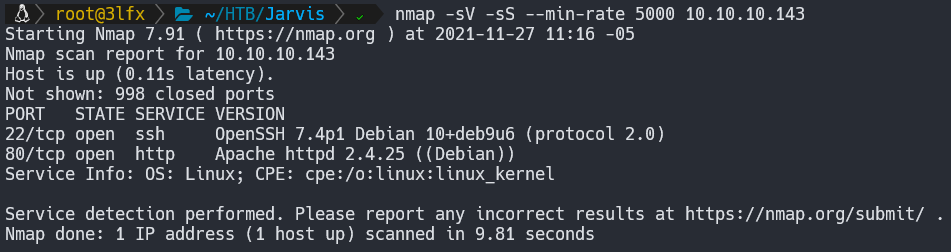
\includegraphics[width=1\textwidth]{imagenes/nmap_jarvis.png} \par \vspace{0.1cm}
            \caption{Escaneo de puertos Jarvis} 
        \end{figure}
    \subsubsection{Análisis de vulnerabilidades y debilidades}
        
=======
\section{Desarrollo de Pruebas de Penetración}
\subsection{HTB01 - Jarvis}
\subsubsection{Escaneo}
Como primera etapa de la Prueba de Penetración realizamos un escaneo de los puertos abiertos por la máquina víctima, encontrando abierto el puerto 22 con el servicio SSH y el puerto 80 con un servicio Web.
\begin{figure}[H]
    \centering
    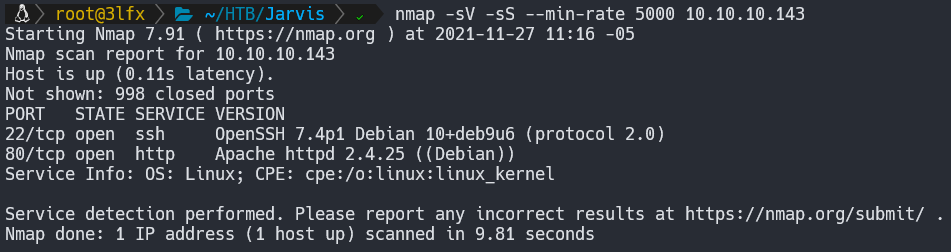
\includegraphics[width=0.99\textwidth]{imagenes/nmap_jarvis.png}
    \caption{Escaneo de puertos en máquina Jarvis}
\end{figure}
\subsubsection{Análisis de Vulnerabilidades}
Al analizar el servicio web, se encontro una página web relacionada a un hotel.
\begin{figure}[H]
    \centering
    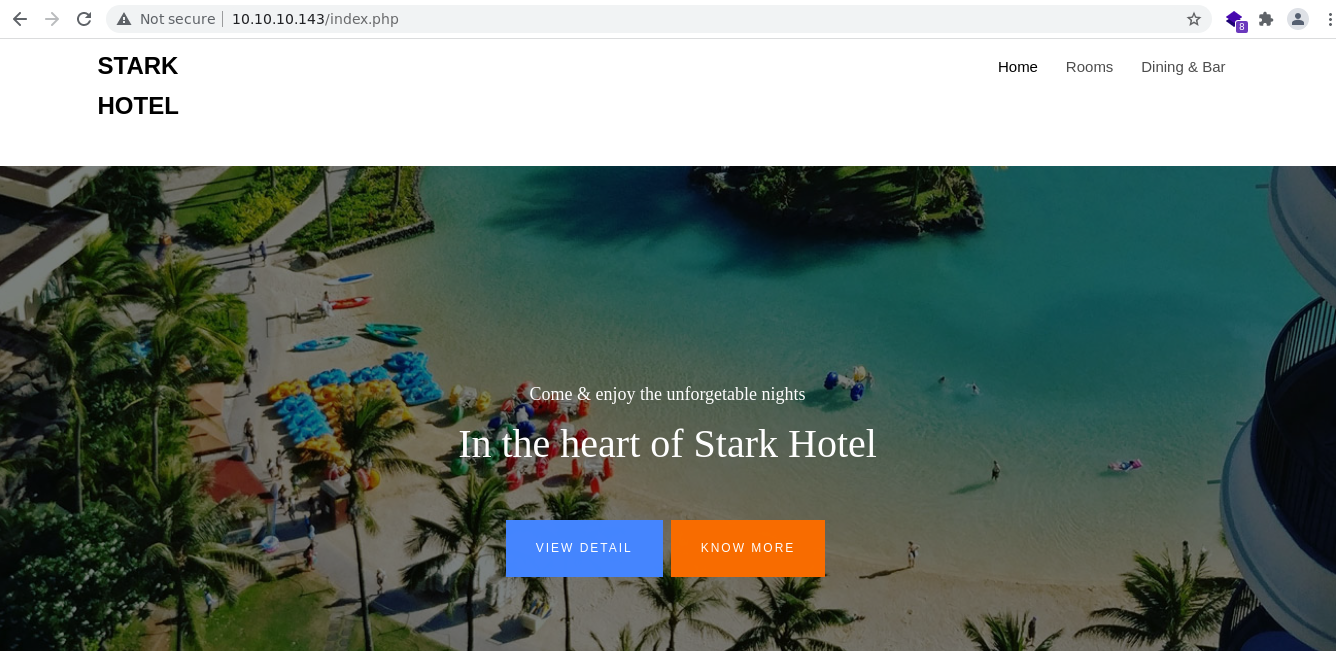
\includegraphics[width=0.99\textwidth]{imagenes/index_jarvis.png}
    \caption{Web Jarvis}
\end{figure}
\subsubsection{Explotación}
\subsubsection{Escalamiento de Privilegios}
\subsubsection{Post-Explotación}
\subsubsection{Recomendaciones de Mitigación}
>>>>>>> f256170ae101aa73e4bc71b5936e56a5d6c15ea0
